% Created by tikzDevice version 0.12.6 on 2025-08-19 18:43:05
% !TEX encoding = UTF-8 Unicode
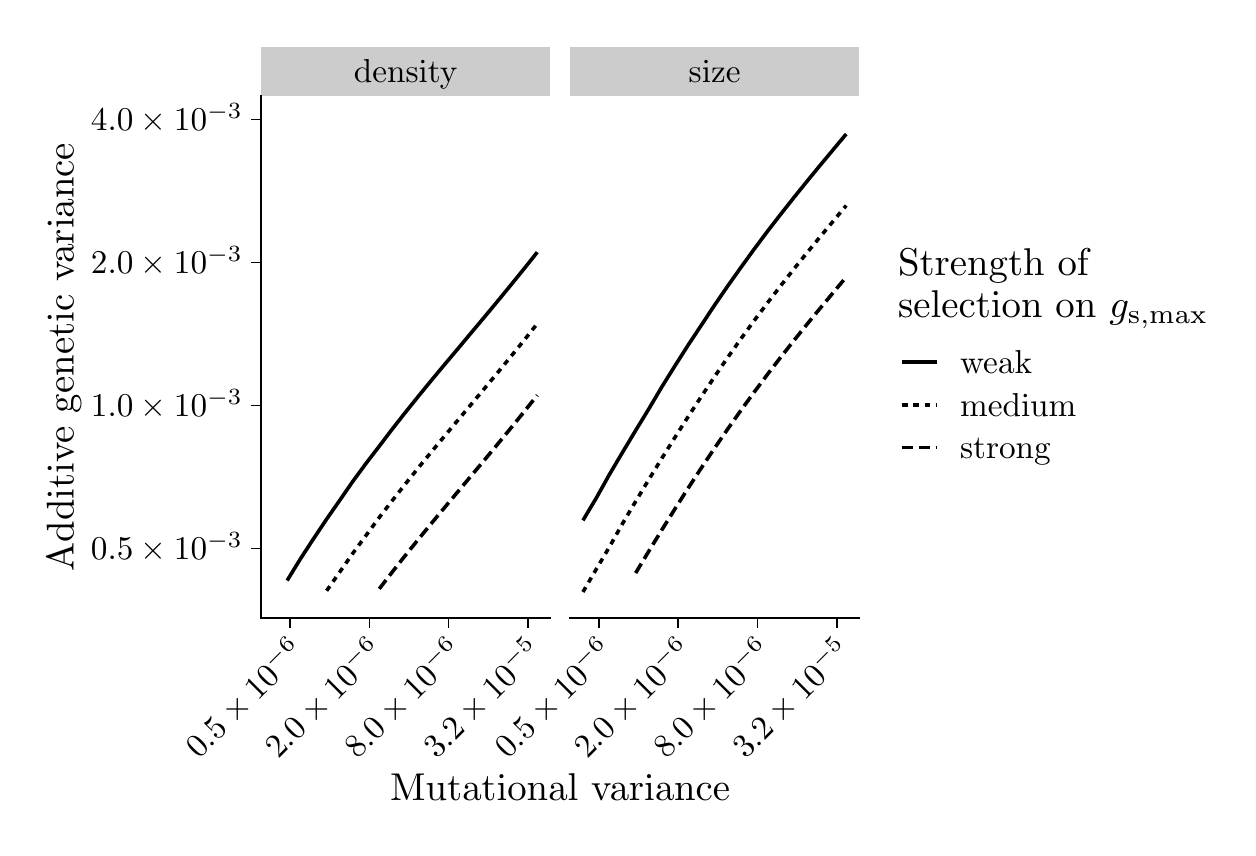
\begin{tikzpicture}[x=1pt,y=1pt]
\definecolor{fillColor}{RGB}{255,255,255}
\path[use as bounding box,fill=fillColor,fill opacity=0.00] (0,0) rectangle (433.62,289.08);
\begin{scope}
\path[clip] ( 84.25, 75.67) rectangle (188.89,264.48);
\definecolor{drawColor}{RGB}{0,0,0}

\path[draw=drawColor,line width= 1.3pt,line join=round] ( 93.76, 89.32) --
	( 98.52, 97.08) --
	(103.27,104.38) --
	(108.03,111.49) --
	(112.79,118.33) --
	(117.54,125.21) --
	(122.30,131.67) --
	(127.06,137.87) --
	(131.81,144.12) --
	(136.57,150.16) --
	(141.33,156.08) --
	(146.08,161.88) --
	(150.84,167.58) --
	(155.60,173.23) --
	(160.35,178.92) --
	(165.11,184.59) --
	(169.87,190.32) --
	(174.62,196.11) --
	(179.38,201.97) --
	(184.14,207.94);

\path[draw=drawColor,line width= 1.3pt,dash pattern=on 2pt off 2pt ,line join=round] (108.03, 85.61) --
	(112.79, 92.42) --
	(117.54, 99.22) --
	(122.30,105.64) --
	(127.06,112.13) --
	(131.81,118.27) --
	(136.57,124.31) --
	(141.33,130.25) --
	(146.08,136.02) --
	(150.84,141.74) --
	(155.60,147.41) --
	(160.35,153.08) --
	(165.11,158.75) --
	(169.87,164.47) --
	(174.62,170.26) --
	(179.38,176.13) --
	(184.14,182.11);

\path[draw=drawColor,line width= 1.3pt,dash pattern=on 4pt off 2pt ,line join=round] (127.06, 86.31) --
	(131.81, 92.48) --
	(136.57, 98.50) --
	(141.33,104.39) --
	(146.08,110.18) --
	(150.84,115.90) --
	(155.60,121.58) --
	(160.35,127.24) --
	(165.11,132.92) --
	(169.87,138.65) --
	(174.62,144.43) --
	(179.38,150.30) --
	(184.14,156.27);
\end{scope}
\begin{scope}
\path[clip] (195.89, 75.67) rectangle (300.54,264.48);
\definecolor{drawColor}{RGB}{0,0,0}

\path[draw=drawColor,line width= 1.3pt,line join=round] (200.65,111.05) --
	(205.41,119.01) --
	(210.16,127.53) --
	(214.92,135.59) --
	(219.68,143.51) --
	(224.43,151.29) --
	(229.19,159.34) --
	(233.95,166.98) --
	(238.70,174.43) --
	(243.46,181.62) --
	(248.22,188.82) --
	(252.97,195.74) --
	(257.73,202.44) --
	(262.49,209.02) --
	(267.24,215.37) --
	(272.00,221.53) --
	(276.76,227.55) --
	(281.51,233.44) --
	(286.27,239.24) --
	(291.03,244.96) --
	(295.78,250.64);

\path[draw=drawColor,line width= 1.3pt,dash pattern=on 2pt off 2pt ,line join=round] (200.65, 85.17) --
	(205.41, 93.32) --
	(210.16,101.35) --
	(214.92,109.84) --
	(219.68,117.87) --
	(224.43,125.76) --
	(229.19,133.53) --
	(233.95,141.13) --
	(238.70,148.58) --
	(243.46,155.86) --
	(248.22,162.99) --
	(252.97,169.93) --
	(257.73,176.65) --
	(262.49,183.17) --
	(267.24,189.52) --
	(272.00,195.69) --
	(276.76,201.72) --
	(281.51,207.62) --
	(286.27,213.41) --
	(291.03,219.12) --
	(295.78,224.80);

\path[draw=drawColor,line width= 1.3pt,dash pattern=on 4pt off 2pt ,line join=round] (219.68, 92.00) --
	(224.43, 99.88) --
	(229.19,107.66) --
	(233.95,115.28) --
	(238.70,122.75) --
	(243.46,130.05) --
	(248.22,137.16) --
	(252.97,144.07) --
	(257.73,150.80) --
	(262.49,157.34) --
	(267.24,163.68) --
	(272.00,169.86) --
	(276.76,175.88) --
	(281.51,181.78) --
	(286.27,187.57) --
	(291.03,193.29) --
	(295.78,198.96);
\end{scope}
\begin{scope}
\path[clip] ( 84.25,264.48) rectangle (188.89,282.08);
\definecolor{fillColor}{gray}{0.80}

\path[fill=fillColor] ( 84.25,264.48) rectangle (188.89,282.08);
\definecolor{drawColor}{RGB}{0,0,0}

\node[text=drawColor,anchor=base,inner sep=0pt, outer sep=0pt, scale=  1.20] at (136.57,269.15) {density};
\end{scope}
\begin{scope}
\path[clip] (195.89,264.48) rectangle (300.54,282.08);
\definecolor{fillColor}{gray}{0.80}

\path[fill=fillColor] (195.89,264.48) rectangle (300.54,282.08);
\definecolor{drawColor}{RGB}{0,0,0}

\node[text=drawColor,anchor=base,inner sep=0pt, outer sep=0pt, scale=  1.20] at (248.22,269.15) {size};
\end{scope}
\begin{scope}
\path[clip] (  0.00,  0.00) rectangle (433.62,289.08);
\definecolor{drawColor}{RGB}{0,0,0}

\path[draw=drawColor,line width= 0.6pt,line join=round,line cap=rect] ( 84.25, 75.67) --
	(188.89, 75.67);
\end{scope}
\begin{scope}
\path[clip] (  0.00,  0.00) rectangle (433.62,289.08);
\definecolor{drawColor}{RGB}{0,0,0}

\path[draw=drawColor,line width= 0.6pt,line join=round] ( 94.82, 72.17) --
	( 94.82, 75.67);

\path[draw=drawColor,line width= 0.6pt,line join=round] (123.46, 72.17) --
	(123.46, 75.67);

\path[draw=drawColor,line width= 0.6pt,line join=round] (152.10, 72.17) --
	(152.10, 75.67);

\path[draw=drawColor,line width= 0.6pt,line join=round] (180.73, 72.17) --
	(180.73, 75.67);
\end{scope}
\begin{scope}
\path[clip] (  0.00,  0.00) rectangle (433.62,289.08);
\definecolor{drawColor}{RGB}{0,0,0}

\node[text=drawColor,rotate= 45.00,anchor=base east,inner sep=0pt, outer sep=0pt, scale=  1.20] at (100.66, 63.32) {$0.5 \times 10^{-6}$};

\node[text=drawColor,rotate= 45.00,anchor=base east,inner sep=0pt, outer sep=0pt, scale=  1.20] at (129.30, 63.32) {$2.0 \times 10^{-6}$};

\node[text=drawColor,rotate= 45.00,anchor=base east,inner sep=0pt, outer sep=0pt, scale=  1.20] at (157.94, 63.32) {$8.0 \times 10^{-6}$};

\node[text=drawColor,rotate= 45.00,anchor=base east,inner sep=0pt, outer sep=0pt, scale=  1.20] at (186.58, 63.32) {$3.2 \times 10^{-5}$};
\end{scope}
\begin{scope}
\path[clip] (  0.00,  0.00) rectangle (433.62,289.08);
\definecolor{drawColor}{RGB}{0,0,0}

\path[draw=drawColor,line width= 0.6pt,line join=round,line cap=rect] (195.89, 75.67) --
	(300.54, 75.67);
\end{scope}
\begin{scope}
\path[clip] (  0.00,  0.00) rectangle (433.62,289.08);
\definecolor{drawColor}{RGB}{0,0,0}

\path[draw=drawColor,line width= 0.6pt,line join=round] (206.47, 72.17) --
	(206.47, 75.67);

\path[draw=drawColor,line width= 0.6pt,line join=round] (235.11, 72.17) --
	(235.11, 75.67);

\path[draw=drawColor,line width= 0.6pt,line join=round] (263.74, 72.17) --
	(263.74, 75.67);

\path[draw=drawColor,line width= 0.6pt,line join=round] (292.38, 72.17) --
	(292.38, 75.67);
\end{scope}
\begin{scope}
\path[clip] (  0.00,  0.00) rectangle (433.62,289.08);
\definecolor{drawColor}{RGB}{0,0,0}

\node[text=drawColor,rotate= 45.00,anchor=base east,inner sep=0pt, outer sep=0pt, scale=  1.20] at (212.31, 63.32) {$0.5 \times 10^{-6}$};

\node[text=drawColor,rotate= 45.00,anchor=base east,inner sep=0pt, outer sep=0pt, scale=  1.20] at (240.95, 63.32) {$2.0 \times 10^{-6}$};

\node[text=drawColor,rotate= 45.00,anchor=base east,inner sep=0pt, outer sep=0pt, scale=  1.20] at (269.59, 63.32) {$8.0 \times 10^{-6}$};

\node[text=drawColor,rotate= 45.00,anchor=base east,inner sep=0pt, outer sep=0pt, scale=  1.20] at (298.23, 63.32) {$3.2 \times 10^{-5}$};
\end{scope}
\begin{scope}
\path[clip] (  0.00,  0.00) rectangle (433.62,289.08);
\definecolor{drawColor}{RGB}{0,0,0}

\path[draw=drawColor,line width= 0.6pt,line join=round,line cap=rect] ( 84.25, 75.67) --
	( 84.25,264.48);
\end{scope}
\begin{scope}
\path[clip] (  0.00,  0.00) rectangle (433.62,289.08);
\definecolor{drawColor}{RGB}{0,0,0}

\node[text=drawColor,anchor=base east,inner sep=0pt, outer sep=0pt, scale=  1.20] at ( 77.75, 96.75) {$0.5 \times 10^{-3}$};

\node[text=drawColor,anchor=base east,inner sep=0pt, outer sep=0pt, scale=  1.20] at ( 77.75,148.42) {$1.0 \times 10^{-3}$};

\node[text=drawColor,anchor=base east,inner sep=0pt, outer sep=0pt, scale=  1.20] at ( 77.75,200.10) {$2.0 \times 10^{-3}$};

\node[text=drawColor,anchor=base east,inner sep=0pt, outer sep=0pt, scale=  1.20] at ( 77.75,251.77) {$4.0 \times 10^{-3}$};
\end{scope}
\begin{scope}
\path[clip] (  0.00,  0.00) rectangle (433.62,289.08);
\definecolor{drawColor}{RGB}{0,0,0}

\path[draw=drawColor,line width= 0.6pt,line join=round] ( 80.75,100.88) --
	( 84.25,100.88);

\path[draw=drawColor,line width= 0.6pt,line join=round] ( 80.75,152.56) --
	( 84.25,152.56);

\path[draw=drawColor,line width= 0.6pt,line join=round] ( 80.75,204.23) --
	( 84.25,204.23);

\path[draw=drawColor,line width= 0.6pt,line join=round] ( 80.75,255.90) --
	( 84.25,255.90);
\end{scope}
\begin{scope}
\path[clip] (  0.00,  0.00) rectangle (433.62,289.08);
\definecolor{drawColor}{RGB}{0,0,0}

\node[text=drawColor,anchor=base,inner sep=0pt, outer sep=0pt, scale=  1.40] at (192.39,  9.72) {Mutational variance};
\end{scope}
\begin{scope}
\path[clip] (  0.00,  0.00) rectangle (433.62,289.08);
\definecolor{drawColor}{RGB}{0,0,0}

\node[text=drawColor,rotate= 90.00,anchor=base,inner sep=0pt, outer sep=0pt, scale=  1.40] at ( 16.64,170.07) {Additive genetic variance};
\end{scope}
\begin{scope}
\path[clip] (  0.00,  0.00) rectangle (433.62,289.08);
\definecolor{drawColor}{RGB}{0,0,0}

\node[text=drawColor,anchor=base west,inner sep=0pt, outer sep=0pt, scale=  1.40] at (314.54,199.41) {Strength of};

\node[text=drawColor,anchor=base west,inner sep=0pt, outer sep=0pt, scale=  1.40] at (314.54,184.29) {selection on $g_\mathrm{s,max}$};
\end{scope}
\begin{scope}
\path[clip] (  0.00,  0.00) rectangle (433.62,289.08);
\definecolor{drawColor}{RGB}{0,0,0}

\path[draw=drawColor,line width= 1.3pt,line join=round] (316.08,168.23) -- (328.40,168.23);
\end{scope}
\begin{scope}
\path[clip] (  0.00,  0.00) rectangle (433.62,289.08);
\definecolor{drawColor}{RGB}{0,0,0}

\path[draw=drawColor,line width= 1.3pt,dash pattern=on 2pt off 2pt ,line join=round] (316.08,152.83) -- (328.40,152.83);
\end{scope}
\begin{scope}
\path[clip] (  0.00,  0.00) rectangle (433.62,289.08);
\definecolor{drawColor}{RGB}{0,0,0}

\path[draw=drawColor,line width= 1.3pt,dash pattern=on 4pt off 2pt ,line join=round] (316.08,137.43) -- (328.40,137.43);
\end{scope}
\begin{scope}
\path[clip] (  0.00,  0.00) rectangle (433.62,289.08);
\definecolor{drawColor}{RGB}{0,0,0}

\node[text=drawColor,anchor=base west,inner sep=0pt, outer sep=0pt, scale=  1.20] at (336.94,164.10) {weak};
\end{scope}
\begin{scope}
\path[clip] (  0.00,  0.00) rectangle (433.62,289.08);
\definecolor{drawColor}{RGB}{0,0,0}

\node[text=drawColor,anchor=base west,inner sep=0pt, outer sep=0pt, scale=  1.20] at (336.94,148.70) {medium};
\end{scope}
\begin{scope}
\path[clip] (  0.00,  0.00) rectangle (433.62,289.08);
\definecolor{drawColor}{RGB}{0,0,0}

\node[text=drawColor,anchor=base west,inner sep=0pt, outer sep=0pt, scale=  1.20] at (336.94,133.30) {strong};
\end{scope}
\end{tikzpicture}
